% Template: LaTeX file for ICMC 2010 papers, with hyper-references
%
% derived from the DAFx-06 templates
% derived from the ICMC 2009 templates by Steve Beck
%
% 1) Please compile using latex or pdflatex.
% 2) Please use figures in vectorial format (.pdf); .png or .jpg are working otherwise 
% 3) Please use the "papertitle" and "pdfauthor" commands defined below

%------------------------------------------------------------------------------------------
\documentclass[twoside,10pt]{article}
\usepackage{icmc2010,amssymb,amsmath} 
%\setcounter{page}{1}

\usepackage{mathptmx} 
\usepackage{rail}

\newcommand{\emptytseg}		{\ensuremath{\oslash}}
\newcommand{\seg}[1]			{Seg(#1)}
\newcommand{\lra}			{$\leftrightarrow$}
\newcommand{\comment}[1]		{\small{[commentaire: #1]}}
\newcommand{\osc}[1]			{{\small\texttt{#1}}}
\newcommand{\rshift}			{\hspace*{4mm}}


%____________________________________________________________
%  !  !  !  !  !  !  !  !  !  !  !  ! user defined variables  !  !  !  !  !  !  !  !  !  !  !  !  !  !
%==== set the title ====
\def\papertitle{Time Synchronization in Graphic Domain - A New Paradigm for Augmented Music Scores}

%==== final submission: author name and affiliation ====
%---- uncomment 1 to 4 lines, for 1 to 4 authors
\def\paperauthorA{D. Fober}
\def\paperauthorB{C. Daudin}
\def\paperauthorC{Y. Orlarey}
\def\paperauthorD{S. Letz}

%-- 4 authors with same affiliation
\affiliation{\paperauthorA, \paperauthorB, \paperauthorC, \paperauthorD}
  {Grame\\ Centre national de cr\'eation musicale, Lyon, France \\ 
  {\tt{{\small \{fober,daudin,orlarey,letz\}@grame.fr}}}}


%  ^  ^  ^  ^  ^  ^  ^  ^  ^  ^ user defined variables  ^  ^  ^  ^  ^  ^  ^  ^  ^  ^  ^  ^ 
%------------------------------------------------------------------------------------------

%%-- if using .ps or .eps figure files, they will be converted on the fly
%%-- RMK: for faster LaTeX runs, use it only once after adding new \includegraphics[]{} cmds
%\usepackage{epstopdf}	 

%---- the hyperref package must be last to properly work
\usepackage[pdftex,
       pdftitle={\papertitle},
	pdfauthor={\paperauthorA},
	colorlinks=false,bookmarksnumbered,pdfstartview=XYZ]{hyperref}
%\pdfcompresslevel=9
\usepackage[pdftex]{graphicx}	% for compatible graphics with hyperref
\usepackage[figure,table]{hypcap}	% corrects the hyper-anchor of figures/tables

\title{\papertitle}

%------------------------------------------------------------------------------------------
\begin{document}

\DeclareGraphicsExtensions{.png,.jpg,.pdf} % used graphic file format for pdflatex
    
\maketitle

%------------------------------------------------------------------------------------------
%:abstract
\begin{abstract}
We propose a simple method for synchronization of arbitrary graphic objects, based on their time relations.
This method relies on \emph{segmentation} and \emph{mappings} that are \emph{relations} between segmentations. 
The paper gives a formal description of \emph{segmentations} and \emph{mappings} and presents 
"Interlude", a framework that implements the proposed method under the form of an \emph{augmented music score viewer}, opening a new space to music notation.
\end{abstract}

%=============================================================
\section{Introduction}\label{sec:introduction}

Music notation has a long history and evolved through ages. From the ancient neumes to the contemporary music notation, western culture is rich of the many ways explored to represent the music. From symbolic or prescriptive notations to pure graphic representation \cite{brown}, the music score has always been in constant interaction with the creative and artistic process. 
However, although the music representations have exploded with the advent of computer music \cite{dann93b,selfridge-field97,hewlett01}, the music score, intended to the performer, didn't evolved in proportion to the new music forms. In particular, there is a significant gap between interactive music and the static way it is generally notated.

Music notation by computer has always been and remains a complex task \cite{BIRD84}. Outside the closed commercial world, the most advanced systems, i.e. those trying to go beyond classical western music notation, propose engraving-based solutions \cite{Hamel98,lilypond03}. Although it doesn't aim at producing music scores, the ENP approach \cite{KUUSK06} is the most opened to score extensions due notably to the Lisp language support. But none of the current approaches are suited to dynamic music notation.

Considering that time is a constant and common property of all musical objects, we propose to give a status of music score to any graphic object having required time properties and we name \emph{augmented music score}, the graphic space that provides representation, composition and manipulation of heterogeneous music objects, both in the graphic and time domains. 
The definition of these time and graphic properties defines a whole class of music scores.

Actually, we aim to consider arbitrary graphic objects (music scores, images, text, signal representation...) as possible scores candidates, and to give them a time position and dimension, to transform them into music score elements, which also implies to make the time relations graphically visible. This concern - to organize the graphic space consistently to the time space - which is at the basis of the classic western music notation, has been stirred through the last century of music notation history \cite{boucou}, but also with composing languages due to the very different nature of algorithmic composition. However, this concern is back in recent research \cite{bresson08}, and notably to synchronize various media \cite{baggi09}. 

Synchronization of heterogeneous medias in the graphic domain raises issues related to non-linearity, non-continuity, non-bijectivity. We propose to approach the problem using \emph{segmentation} and the description of relations between \emph{segments} - we will next use the term \emph{mappings} to refer to these relations.

The paper presents the segmentation and mapping formalism. Next, it introduces "Interlude", a framework that implements \emph{augmented music scores}, making use of the segmentation and mapping formalism. Some examples of applications are finally given.


%=============================================================
\section{Segmentation and mappings}\label{sec:segmapping}

\subsection{Definitions}\label{subsec:definitions}

We will first introduce the notions of graphic and time segments. Next we will generalize these concrete definitions in an abstract and generic segment definition.


%-------------------------------------------------------------
\subsubsection{Time Segment}\label{subsec:timeseg}

A \emph{time segment} is an interval
 $i=[t_{0},t_{1}[$ such as $t_{0} \leqslant t_{1}$.
An interval $i=[t_{0},t_{1}[$ is said to be empty when $t_{0} = t_{1}$. We will use the notation \emptytseg\ for the empty time segment.

Intersection between time segments is the largest interval defined as:
%\begin{equation}
\[ 
\forall i,\ \forall  j, 
\ i \cap j  := i' \ |\ \forall t \in i'\  t \in i \ \land\ t \in j   
\]
%\end{equation}


%-------------------------------------------------------------
\subsubsection{Graphic Segment}\label{subsec:graphicseg}
A \emph{graphic segment} is defined as a set of two intervals $\{g_x,g_y\}$ where $g_x$ is an interval on the x-axis and $g_y$, on the y-axis.

A graphic segment $g=\{g_x,g_y\}$ is said to be empty when $g_x = \emptytseg$ or $g_y = \emptytseg$

Intersection $\cap$ between graphic segments is defined as:
%\begin{equation}
\[ 
\forall g=\{g_x,g_y\},\ \forall  h=\{h_x,h_y\},\ g \cap h = \{g_x \cap h_x,\ g_y \cap h_y\}
\]
%\end{equation}

%-------------------------------------------------------------
\subsubsection{Segment Generalization}\label{subsec:generalseg}

We extend the definitions above to a general definition of a $n$-dimensional segment.
A $n$-dimensional segment is a set of $n$ intervals $s^n=\{i_1,...,i_n\}$ where $i_j$ is an interval on the dimension $j$.

A $n$-dimensional segment $s^n$ is said to be empty when $\exists i \in s^n\ |\ i = \emptytseg $

Intersection between segments is defined as the set of their intervals intersection:
\begin{equation}
%\[ 
s_1^n \cap s_2^n := \{i^j\}\ |\ i^j = i_1^j \cap i_2^j\ \land\  0 \leqslant j < n
%\]
\end{equation}

%=============================================================
%\section{Segmentation and mappings}\label{sec:segmapping}

%-------------------------------------------------------------
\subsection{Resource Segmentation}\label{subsec:resourceseg}

A \emph{segment-able} resource $R$ is a $n$-dimensional resource defined by a $n$-dimensional segment $S^n$.
The segmentation of a resource $R$ is the set of segments
$\seg{R}=\{ s_1^n, ... s_i^n\}$ such as: \\
\begin{displaymath}
\begin{array}{rll}
\forall i, j \in \seg{R} & i \cap j =  \emptytseg  & $the segments are disjoints$ \\
\forall i \in \seg{R} & i \cap S^n = i & $segments are included in R$ \\
\end{array}
\end{displaymath}


%-------------------------------------------------------------
\subsection{Mapping}\label{subsec:mapping}

A \emph{mapping} is a relation between \emph{segmentations}.

For a mapping $M\subseteq \seg{R_{1}}\times \seg{R_{2}}$ we define two functions:
\begin{equation}
%\[ 
M^{+}(i)=\{ i'\in \seg{R_{2}}\ |\ (i,i')\in M\}
%\]
\end{equation}
that gives the set of segments from $R_{2}$ associated to the segment
$i$ from $R_{1}$. 

and the reverse function:
\begin{equation}
%\[ 
M^{-}(i')=\{ i \in \seg{R_{1}}\ |\ (i,i')\in M\}
%\]
\end{equation}
that gives the set of segments from $R_{1}$ associated to the segment $i'$ from $R_{2}$.


%----------------------------------------------------------------
\subsection{Mappings composition}\label{subsec:compmap}
Mappings composition is quite straightforward.\\
For a mapping $M_{1}\subseteq \seg{R_{1}}\times \seg{R_{2}}$ \\
and a mapping $M_{2}\subseteq \seg{R_{2}}\times \seg{R_{3}}$, then :
\[ M_{1} \circ M_{2} \subseteq \seg{R_{1}}\times \seg{R_{3}} \]


%=============================================================
\section{Augmented Music Score}\label{sec:augmscore}

Augmented music scores have been developed in the framework of the Interlude project\footnote{Interlude - ANR-08-CORD-010}, which objective is to investigate gestural interaction with music content, both in the audio and symbolic domains.

An augmented score is a graphic space that provides representation, composition and manipulation of heterogeneous music objects, both in the graphic and time domains. It supports arbitrary resources like music scores, images, text, vectorial graphics and signals representations (not detailed in this paper). It focuses on the graphic synchronization of its components, according to their time relations.

%-------------------------------------------------------------
\subsection{The Interlude Library}\label{sec:itl}

Augmented score capabilities are provided under the form of a C++ platform independent library. 
It supports the Guido \cite{hoos98} and the MusicXML formats \cite{good01} as music notation input. It makes use to the Guido Engine \cite{Fober:04b,RENZ02} for the score layout and relies on the Qt framework \cite{qt4} for the rendering of the other resource types and to ensure platform independence. All of the library features are available as C++ API as well using OSC \cite{OSC} messages.

%-------------------------------------------------------------
\subsection{Augmented Score Segmentations and Mappings}\label{sec:asm}

All the resources that are part of an augmented score have a graphic dimension and a temporal dimension in common. Thus, they are \emph{segment-able} in the graphic and time spaces. Unless specified otherwise, time is referring to music time (i.e. metronomic time). 

In  addition, each resource type is \emph{segment-able} in its specific space: audio frames linear space for an audio signal, two dimensional space organized in lines/columns for text, etc.

\begin{table}[htdp]
\begin{center}
\begin{tabular}{|r|l|}
\hline
type & segmentations and mappings required \\
\hline
text		& \textit{graphic} \lra\ \textbf{text  \lra\ time} \\
score		& \textit{graphic \lra\ wrapped time} \lra\ \textit{time} \\
image		& \textit{graphic} \lra\ \textbf{pixel \lra\ time} \\
vectorial graphic	&  \textit{graphic} \lra\ \textbf{vectorial \lra\ time} \\
signal		&  \textit{graphic} \lra\ \textbf{frame \lra\ time} \\
\hline
\end{tabular}
\end{center}
\caption{Segmentations and mappings for each component type}
\label{maptable}
\end{table}

Table \ref{maptable} lists the segmentations and mappings used by the different component types. Mappings are indicated by arrows (\lra). Note that the arrows link segments of different types (the \emph{segment} qualifier is omitted). Segmentations and mappings in  \textit{italic} are automatically computed by the system, those in \textbf{bold} must be given externally. This typology could be extended to any kind of resource, provided that a mapping exists to go from the graphic space to the time space. 

Note that for music scores, an intermediate time segmentation, the \emph{wrapped time}, is necessary to catch repeated sections and jumps (to sign, to coda, etc.).

Composing these mappings is at the basis of the mechanisms to address and synchronize the components both in the graphic and time spaces.

%------------------------------------------------------------
\subsection{Time to graphic conversion and synchronization}


Let's consider two score components $A$ and $B$ with their corresponding graphic and time segmentations:\\
\rshift $\seg{A_g}$, $\seg{A_t}$, $\seg{B_g}$, $\seg{B_t}$. \\
In addition, $B$ has an intermediate segmentation $\seg{B_l}$ expressed in the resource local space units (e.g. frames for an audio signal).
The mappings \\
\rshift $M_A \subseteq \seg{A_{g}}\times \seg{A_{t}}$ and $M_B \subseteq \seg{B_{t}}\times \seg{B_{l}}$ \\
give the correspondence between graphic and time space for $A$ and between time and local space for $B$.

When synchronizing objects and to decide on what position should be used as base position, the Interlude library introduces a master/slave relation between components: a slave is constrained to its master graphic space.

%------------------------------------------------------------
\subsubsection{Graphic alignment of time positions}

Let's consider that $B$ is $A$ slave and that we want to graphically align $B$ to $A$ at a time $t$. Let $s=[s_0, s_1[$ be the $A$ segment containing the time $t$. Then the corresponding graphic segment is:
\[
M_A^{-}(s) =\{ g \in \seg{A_{g}}\ |\ (g,s)\in M_A\}
\]
For each $M_A^{-}(s)$ segment, $B$ graphic position can be computed by simple linear interpolation i.e.:
\[
(x_B, y_B) = (g_{x0} + (g_{x1} - g_{x0}). \delta,\ g_{y0})
\]
where $g_{x0}$ and $g_{x1}$ are the graphic segment first and last $x$ coordinates and 
$\delta = (t - s_0) / (s_1 - s_0)$.
%$\delta = \frac{t - s_0}{s_1 - s_0}$.

$y_B$ is arbitrary fixed to $g_{y0}$ but it is actually controlled by a synchronization mode (over, above, below).

%When $s$ is mapped to several graphic segments, additional information may be required to select a final target segment.

%------------------------------------------------------------
\subsubsection{Segments graphic alignment}
The basic principle of segments alignment consists for each of the master graphic segment, to retrieve the corresponding slave segment expressed in the slave local coordinates and to render this slave segment in the space of the master graphic segment.
Provided that $\seg{A_t} = \seg{B_t}$, the operation may be viewed as the mapping composition 
\[
M_{A} \circ M_{B} \subseteq \seg{A_{g}}\times \seg{B_{l}}
\]
Figure \ref{fig:align} gives an example of a bitmap aligned to different score locations.
\begin{figure}[htbp]
\centerline{
	\framebox{
	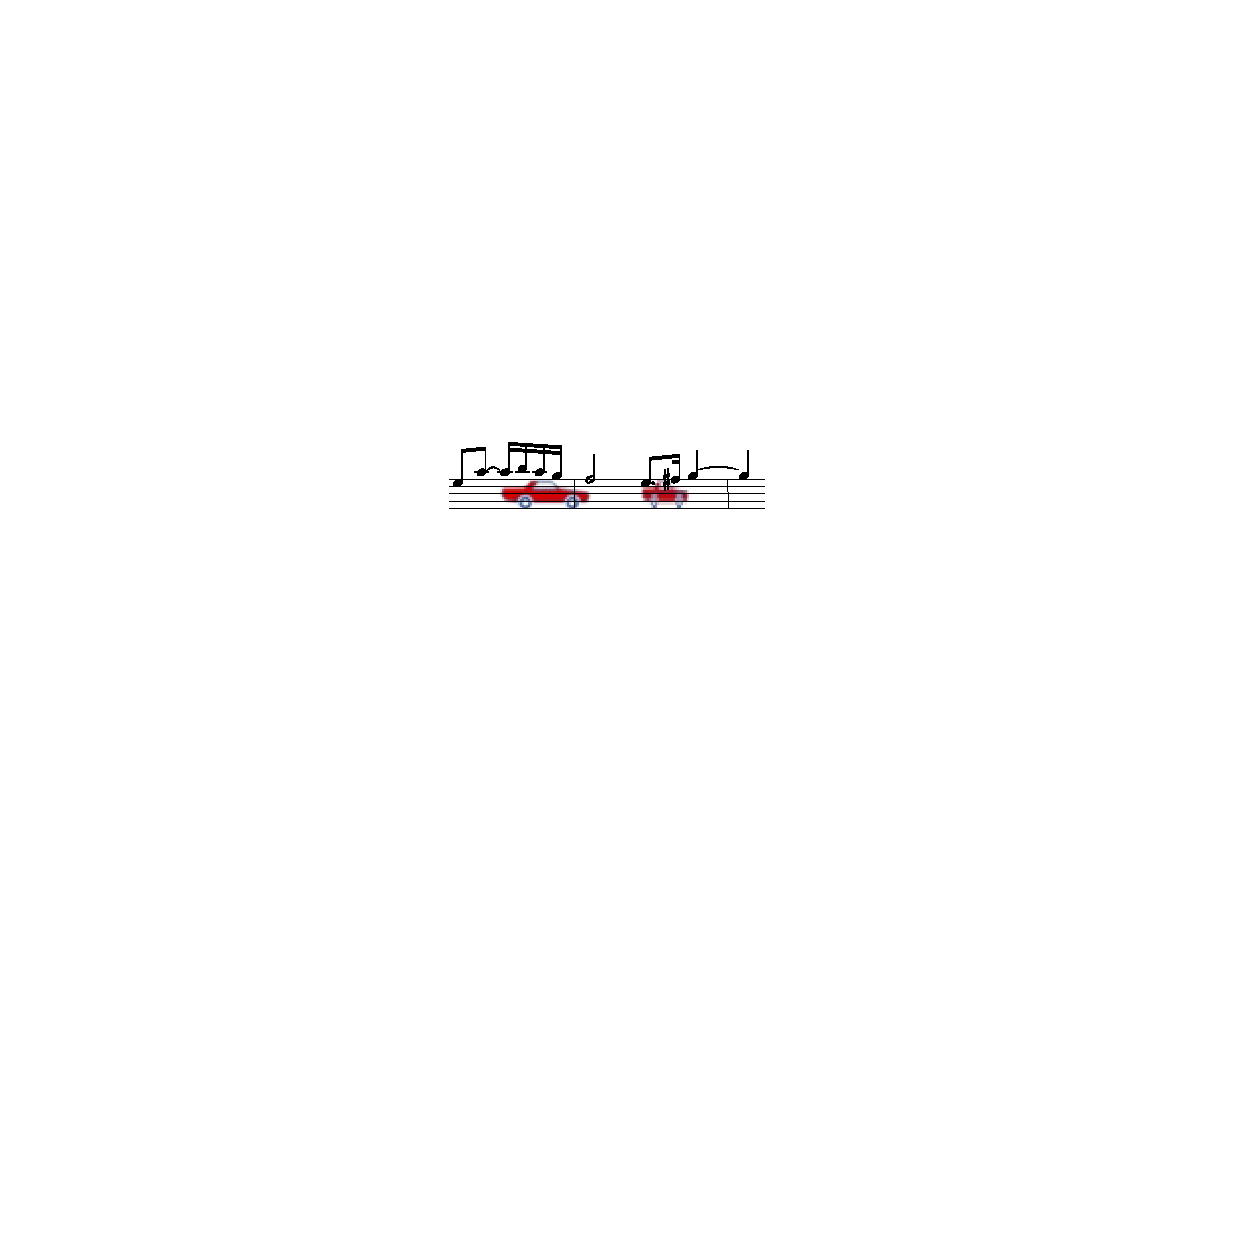
\includegraphics[width=0.6\columnwidth]{imgs/synccars}}
	}
\caption{The same car bitmap synchronized to different time positions. The car has a quarter note duration, it is stretched to the corresponding score graphic segments.}
\label{fig:align}
\end{figure}

%=============================================================
\subsection{The Interlude viewer}

The Interlude viewer is build on top of the Interlude library. It has no user interface since it has been primarily designed to be controlled via OSC messages i.e. using external applications like Max/MSP or Pure Data.

\subsubsection{Messages general format}

An Interlude OSC message is made of an OSC address, followed by a message string, followed by $0$ to $n$ parameters. The message string could be viewed as the method name of the object identified by the OSC address. The OSC address is a string or a regular expression matching several objects.
The OSC address space includes predefined static nodes:\\
\rshift \osc{/ITL} corresponds to the Interlude viewer application \\
\rshift \osc{/ITL/scene} corresponds to the rendering scene, actually the augmented score address.

The next section presents an example of OSC messages setting up a score including synchronized components. Note that the messages list corresponds strictly to the file format of a score. Note also that this example is static while real-time interaction is always possible, for example to move objects in time by sending \osc{clock} or \osc{date} messages.


\subsubsection{Nested synchronization example}

This example uses 3 components; the first one is master of the second, which is master of the third one. Lines beginning with a '\#' are comments interleaved with the messages.

{\small \begin{verbatim}
# creates a score using an image
/ITL/scene/score set img "score.jpg"
# sets the score graphic to time mapping 
/ITL/scene/score mapf "score.map"

# creates a text using a text file
/ITL/scene/text set txtf "comment.txt"
# changes the text scale
/ITL/scene/text scale 3.0
# and the text color
/ITL/scene/text color 0 0 240 255
# put the text in front
/ITL/scene/text z 0.5
# and sets the text to time mapping 
/ITL/scene/text mapf "comment.map"

# creates a ball as vectorial graphic
/ITL/scene/ball set ellipse 0.2 0.2
# puts it in front
/ITL/scene/ball z 0.4
# changes the ball color
/ITL/scene/ball color 250 50 0 255

# sets all the objects date
/ITL/scene/* date 4 1
# sets the text slave of the score
/ITL/scene/sync text score
# sets the ball slave of the text
/ITL/scene/sync ball text
\end{verbatim}
}Note the use of a wildcard in the OSC address to set all the objects date with a single message. 
The corresponding result is given by figure \ref{fig:scene}.

\begin{figure}[htbp]
\centerline{\framebox{
	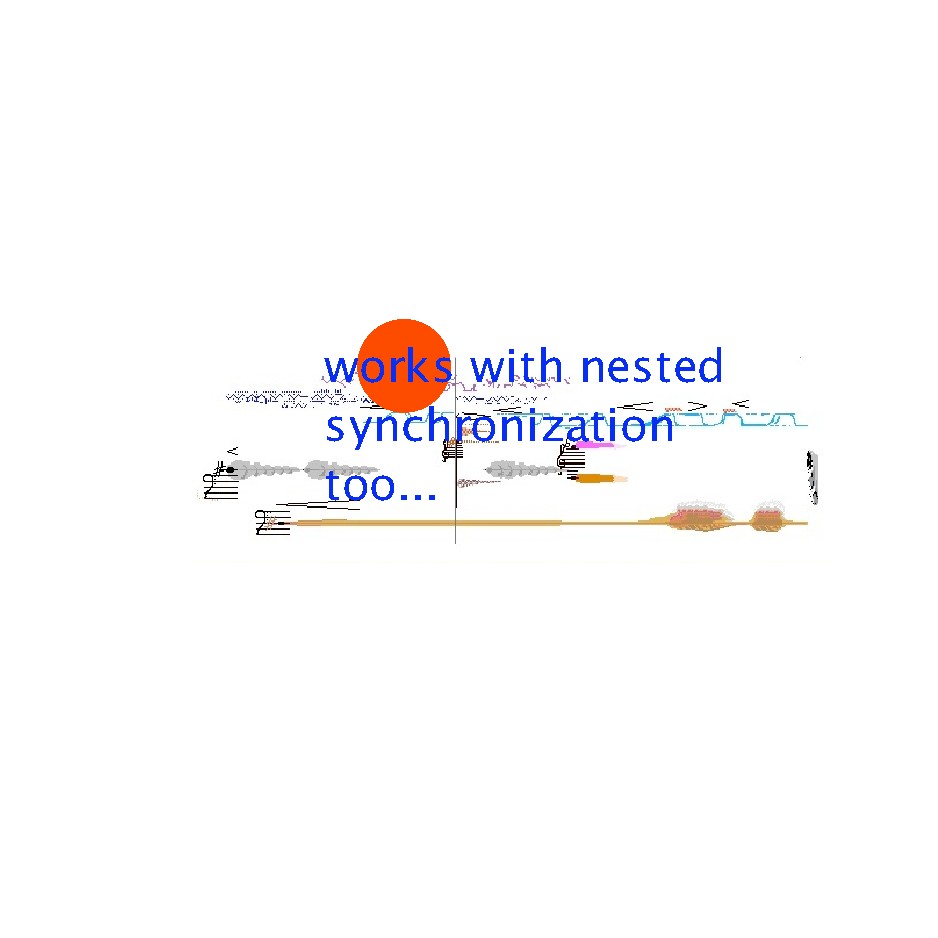
\includegraphics[width=0.9\columnwidth]{imgs/scene}}}
\caption{A score with nested synchronization.}
\label{fig:scene}
\end{figure}

%=============================================================
\section{Conclusion}

The proposed method for synchronizing arbitrary objects in the graphic space according to their time relations combines the advantages of simplicity and flexibility: a great variety of behaviors may be obtained depending on the defined segmentations and mappings. There are many potential application domains, including pedagogic applications, games, but also new music forms like interactive music.

%=============================================================
\vspace{4mm}
\hspace{-6mm}
\textbf{Acknowledgments} \\
The Interlude project is funded by the Agence Nationale pour la Recherche [ANR-08-CORD-010].


\bibliographystyle{IEEEtranS}
\bibliography{icmc2010}

\end{document}

